%!TEX TX-program = xelatex
\documentclass[8pt]{article}

\usepackage{ctex}
\usepackage{graphicx}
\usepackage{enumitem}
\usepackage{geometry}
\usepackage{amsmath}
\usepackage{amssymb}
\usepackage{amsfonts}
\usepackage{tikz}
\usepackage{extarrows}
\usetikzlibrary{positioning}
\usetikzlibrary{svg.path}
\usepackage{xcolor}
\usepackage{soul}

\graphicspath{ {./images/} }

\author{高一(6)班\ 邵亦成\ 26号}
\title{12 函数综合(难题)}
\date{2021年12月8日}

\geometry{a4paper, scale=0.8}

\begin{document}

	\maketitle

	\begin{enumerate}[label=\arabic*.]
		\item 设区间$[a, b]$是函数$f(x)$的定义域$D$的子集, 定义在$[a, b]$上的函数$g(x)=|f(x)-f(x_0)| (x_0 \in [a, b])$记为$g_{[a, b]}(x, x_0)=|f(x)-f(x_0)|.$ 若$f(x)=\displaystyle \left\{\begin{array}{rl}2\sqrt{x}, &0\leq x<1,\\\frac{1}{x}, &x\geq 1.\end{array}\right.$
			\begin{enumerate}[label=(\arabic*)]
				\item 求$f(x)$的值域.
					~\\

					考虑$x\in[0, 2)$, $f(x)=2\sqrt{x}\in[0, 2).$

					考虑$x\in[1, +\infty)$, $f(x)=\dfrac{1}{x}\in(0, 1]$.

					故$f(x)$的值域为$[0, 2)$.

				~\\

				\item 关于$x$的方程$g_{[0, 4]}(x, 2)-t=0$恰有3个不同的解时, 求实数$t$的取值范围.
					~\\

					$$g_{[0, 4]}(x, 2)-t=0\Leftrightarrow \left|f(x)-\frac{1}{2}\right|=t, x\in[0, 4].$$

					令

					\begin{align*}
					F(x) &= \left|f(x)-\frac{1}{2}\right|\\
					     &= \left\{\begin{array}{rl}\dfrac{1}{2}-2\sqrt{x},&0\leq x\leq \dfrac{1}{16},\\\\2\sqrt{x}-\dfrac{1}{2},&\dfrac{1}{16}<x<1,\\\\\dfrac{1}{x}-\dfrac{1}{2},&1\leq x\leq 2,\\\\\dfrac{1}{2}-\dfrac{1}{x},&2<x\leq 4.\end{array}\right.
					\end{align*}

					绘制函数$y=F(x)$的图像, 如下图:

					$$
					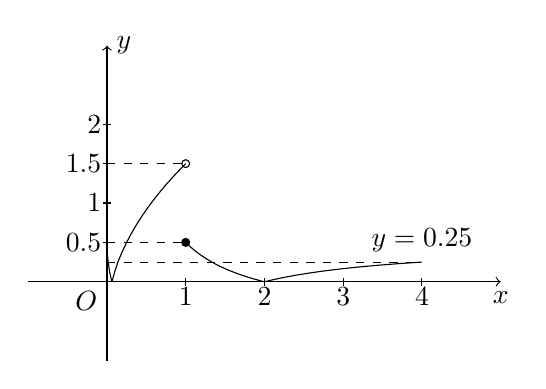
\begin{tikzpicture}[scale=1]
			    		\draw[black, ->] (-1,  0)--( 5,  0) node[below] {$x$};
			    		\draw[black, ->] ( 0, -1)--( 0, 3) node[right] {$y$} node at (0, 0) [anchor=north east] {$O$};
    					\foreach \x/\xtext in {1/1, 2/2, 3/3, 4/4}{
    						\draw (\x, -0.05) -- (\x, 0.05) node[below] {\xtext};
    					}
    					\foreach \y/\ytext in {0.5/0.5, 1/1, 1.5/1.5, 2/2}{
    						\draw (-0.05, \y) -- (0.05, \y) node[left] {\ytext};
    					}
			    		\draw[black, domain=0:1/16] plot(\x, {1/2 - 2 * (\x^(1/2))});
			    		\draw[black, domain=1/16:1] plot(\x, {2 * (\x^(1/2)) - (1/2)});
			    		\draw[black] (1, 1.5) circle (0.05);
			    		\filldraw[black] (1, 0.5) circle (0.05);
			    		\draw[black, domain=1:2] plot(\x, {(1/\x) - (1/2)});
			    		\draw[black, domain=2:4] plot(\x, {(1/2) - (1/\x)});
			    		\draw[black, dashed] (0, 1.5)--(1, 1.5);
			    		\draw[black, dashed] (0, 0.5)--(1, 0.5);
			    		\draw[black, dashed] (0, 0.25)--(4, 0.25) node[above] {$y=0.25$};
			    	\end{tikzpicture}
					$$

					故有$t\in\left(\dfrac{1}{4}, \dfrac{1}{2}\right].$

			\end{enumerate}

		~\\

		\item 设$n$为正整数, 规定: $\displaystyle f_n (x) = \underbrace{f\{f[\cdots f(x)\cdots]\}}_{n\text{个}f}$. 已知$f(x)=\left\{\begin{array}{rl}2(1-x), &0\leq x\leq 1,\\x-1, &1<x\leq 2.\end{array}\right.$
			\begin{enumerate}[label=(\arabic*)]
				\item 解不等式: $f(x)\leq x$.
					~\\

					考虑$0\leq x\leq 1$, $2(1-x)\leq x \Rightarrow x\geq \frac{2}{3}$, 即$x\in\left[\dfrac{2}{3}, 1\right]$.

					考虑$1 < x \leq 2$, 不等式恒成立, 即$x\in(1, 2]$.

					故$x\in\left[\dfrac{2}{3}, 2\right]$.

				~\\

				\item 设集合$A=\{0, 1, 2\}$, 对任意$x\in A$, 证明: $f_3(x)=x$.
					~\\

					考虑$x=0$, $f_3(0)=f(f(f(0)))=f(f(2))=f(1)=0$.

					考虑$x=1$, $f_3(1)=f(f(f(1)))=f(f(0))=f(2)=1$.

					考虑$x=2$, $f_3(2)=f(f(f(2)))=f(f(1))=f(0)=2$.

				~\\

				\item 求$f_{2021}\left(\dfrac{8}{9}\right)$的值.
					~\\

					\begin{align*}
						f_1\left(\frac{8}{9}\right) &= 2\left(1-\frac{8}{9}\right)=\dfrac{2}{9},\\
						f_2\left(\dfrac{8}{9}\right) &= f\left(f\left(\frac{9}{9}\right)\right) = f\left(\frac{2}{9}\right) = \frac{14}{9},\\
						f_3\left(\dfrac{8}{9}\right) &= f\left(f_2\left(\frac{9}{9}\right)\right) = f\left(\frac{14}{9}\right) = \frac{5}{9},\\
						f_4\left(\dfrac{8}{9}\right) &= f\left(f_3\left(\frac{9}{9}\right)\right) = f\left(\frac{5}{9}\right) = \frac{8}{9}.\\
					\end{align*}

					一般的, $\forall k, r\in\mathbb{N}$,

					$$f_{4k+r}\left(\frac{8}{9}\right) = f_{r}\left(\frac{8}{9}\right).$$

					故有

					$$f_{2010}\left(\frac{8}{9}\right)=f_2\left(\frac{8}{9}\right)=\frac{14}{9}.$$

			\end{enumerate}

	\end{enumerate}

\end{document}